\section{Chestwall Experiment}
\subsection{Setup}
\label{sec:exp}

The experimental apparatus is shown schematically in Fig.~\ref{fig:schem}.  Briefly, a collimated continuous-wave $785\,{\rm nm}$ laser diode is coupled to a 2D galvanometer scanner (Thorlabs GVS012). The laser beam with a focused spot   size of $0.5 mm$ is raster scanned on a $35\times 35$ square grid
with a $4\,{\rm mm}$ spacing covering a $13.6\times 13.6\,{\rm cm}^2$ area on one side of the imaging tank (whose overall dimensions are $44\times 44\times 6\,{\rm cm}^3$). The thickness of the tank was chosen to be close to the average compression used in our previous clinical studies based on diffuse optical tomography~\cite{choe_09_1, culver_03_1}. As each source position is illuminated, data is collected from the opposite side of the tank over
a $21.2\times 21.2\,{\rm cm}^2$ field of view (FOV) area with a CCD camera (Andor, DV887ECS-UV, lens $25\,{\rm mm}\ {\rm F}/0.95$). The FOV was mapped to the grid of $512\times 512$ CCD pixels. This corresponds to a rectangular grid on the surface of the tank with the spacing $p=0.416\,{\rm mm}$.

\begin{figure}[t]
\centering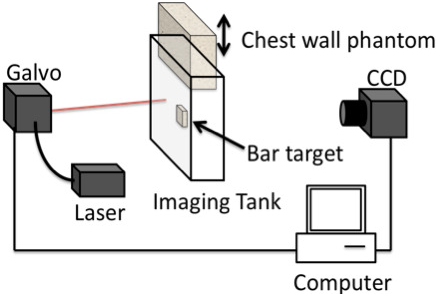
\includegraphics[width=7cm]{./figures/chestwall_1.pdf}
\caption{\label{fig:schem}
  Schematic of the experimental setup. A collimated CW $785\,{\rm nm}$
  laser source at is raster scanned on one side of the imaging tank.
  The transmitted light on the detection plane is collected by a CCD
  for each source position.}
\end{figure}

A bar target is suspended in the mid-plane of the tank ($3\,{\rm cm}$ from either surface) using monofilament fishing line. The target is made of silicon rubber (RTV-12, General Electric), titanium oxide (T-8141, Sigma-Aldrich) and carbon black (Raven 5000 Ultra Powder II), with the absorption coefficient $\mu_{\rm a}=0.2\,{\rm cm}^{-1}$ and the reduced scattering coefficient $\mu_{\rm s}^\prime = 7.5\,{\rm cm}^{-1}$.  The tank is filled with a scattering fluid ($\mu_{\rm a} = 0.05\,{\rm cm}^{-1}$ and $\mu_{\rm s}^\prime = 7.5\,{\rm cm}^{-1}$); these background optical properties are similar to those used in previous {\em in vitro} and clinical research. The contrast between the target and the surrounding fluid is purely absorptive with the ratio of about 4.

A chest wall phantom (Biomimic, INO $\mu_{\rm a} = 0.1\,{\rm cm}^{-1}$ and $\mu_{\rm s}^\prime = 5.0\,{\rm cm}^{-1}$, dimensions $40\times
20\times 5.8\,{\rm cm}^3$) is suspended at various distances $d$ from the top edge of the bar target ($d=2$, $5$, $8$, $11$, $14$, $17\,{\rm
  cm}$). The optical properties of the chest wall phantom were chosen to mimic muscle tissue~\cite{ardeshirpour_10_1, kienle_99_1,taroni_03_1}.  Thus both
absorptive and scattering contrast exists between the chest wall phantom and the background fluid. The bar target and the chest wall phantom are shown in Fig.~\ref{fig:targets}.  Note that the chest wall phantom almost entirely fills the imaging tank; the clearance between the chest wall phantom and the inner surfaces of the tank is $1\,{\rm mm}$ on both sides.

\begin{figure}[t]
  \centering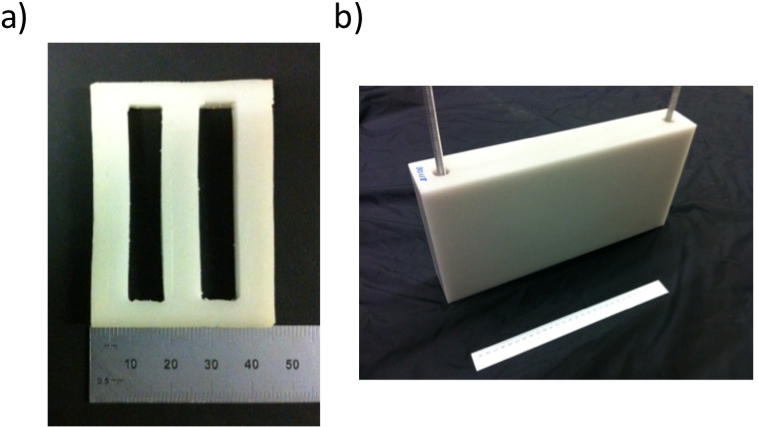
\includegraphics[width=8cm]{./figures/chestwall_2.pdf}
\caption{\label{fig:targets}
  Phantoms used in the experiment.  (a) $6\,{\rm mm}$ thick bar target
  with $\mu_{\rm a}=0.2\,{\rm cm}^{-1}$ and $\mu_{\rm
    s}^{\prime}=7.5\,{\rm cm}^{-1}$ has slots $48\,{\rm mm}$ tall and
  $9\,{\rm mm}$ wide. The outer dimensions are $60\times 50\,{\rm
    mm}^2$. (b) The chest wall phantom with $\mu_{\rm a}=0.1\,{\rm
    cm}^{-1}$ and $\mu_{\rm s}^{\prime}=5.0\,{\rm cm}^{-1}$.  }
\end{figure}


\section{Image reconstruction}
\label{sec:rec}

\subsection{Linearized integral equations}
\label{subsec:lin_eq}

This research employs linear image reconstruction methods and CW data. In principle, one could also resort to time ~\cite{patterson_89_1,benaron_93_1,andersson-engels_90_1,jacques_89_1,schmidt_00_2,ntziachristos_98_1} or frequency-resolved~\cite{gratton_90_1,fishkin_93_1,chance_98_1,pogue_94_1} measurements and nonlinear reconstruction methods~\cite{arridge_99_1,markel_03_2} to obtain a reconstruction of the target and the chest wall phantom simultaneously; however, these approaches require more expensive and complex instrumentation, as well as more time-consuming computational schemes. For our linear approach, two independent measurements of the transmitted intensity are taken, one in a homogeneous (reference) slab and the other in a slab with the target and the chest wall phantom present. We denote these measurements by $I_0({\bf r}_{\rm d}, {\bf r}_{\rm s})$ and $I({\bf r}_{\rm d}, {\bf r}_{\rm s})$, respectively, where ${\bf r}_{\rm d}$ and ${\bf r}_{\rm s}$ are the two-dimensional vectors specifying the lateral positions of the detector and the source on the respective
surfaces of the tank. In this work, $I_0$ and $I$ are expressed in CCD counts. These measurements can be related to the medium optical properties through the relations
%
\begin{equation}
I({\bf r}_{\rm d}, {\bf r}_{\rm s}) =
A({\bf r}_{\rm d})B({\bf r}_{\rm s})G({\bf r}_{\rm d},{\bf r}_{\rm s})
\ , \ \ 
I_0({\bf r}_{\rm d},{\bf r}_{\rm s})=
A({\bf r}_{\rm d})B({\bf r}_{\rm s})G_0({\bf r}_{\rm d},{\bf r}_{\rm
  s}) \ .
\label{eq1}
\end{equation}
%
\noindent
Here $A({\bf r}_{\rm d})$ and $B({\bf r}_{\rm s})$ are unknown coupling coefficients associated with the source and detection system which can be excluded from consideration as described below. $G({\bf r}_{\rm d}, {\bf r}_{\rm s})$ and $G_0({\bf r}_{\rm d}, {\bf r}_{\rm  s})$ are the Green's functions for the diffusion equation in the slab with the inhomogeneities present and in the homogeneous and reference slab, respectively. The latter is known analytically~\cite{markel_04_4}. The two Green's functions are mathematically related by the Dyson equation. Under the assumption that the scattering properties of the medium are spatially uniform, the Dyson equation has the form
%
\begin{equation}
G({\bf r}_{\rm d}, {\bf r}_{\rm s}) = G_0({\bf r}_{\rm d}, {\bf r}_{\rm s}) -
\int_V G_0({\bf r}_{\rm d}, {\bf r}) \delta\alpha({\bf r}) G({\bf r},
{\bf r}_{\rm s})\,d^3r \ .
\label{eq2}
\end{equation}
%
\noindent
Here the integral is taken over the volume of the slab and $\delta\alpha({\bf r}) = c\left[\mu_{\rm a}({\bf r}) - \mu_{{\rm a}0} \right]$ is the deviation of the absorption coefficient at a given point from the background value $c\mu_{{\rm a}0}$, where $c$ is the average speed of light in the medium.

The procedure of linearization consists of making an approximation to Eq.~(\ref{eq2}) so as to exclude the unknown function $G({\bf r}, {\bf  r}_{\rm s})$ from the right-hand side. In the first Rytov approximation~\cite{schotland_97_1}, Eq.~(\ref{eq2}) is rewritten as
%
\begin{equation}
G({\bf r}_{\rm d}, {\bf r}_{\rm s}) = G_0({\bf r}_{\rm d}, {\bf r}_{\rm s})
\exp\left[ -\int_V \frac{G_0({\bf r}_{\rm d}, {\bf r}) \delta\alpha({\bf r})
G({\bf r}, {\bf r}_{\rm s}) \,d^3r}{G_0({\bf r}_{\rm d}, {\bf r}_{\rm s})}
\right] \ .
\label{eq3}
\end{equation}
%
\noindent
Consequently, we define the data function $\phi({\bf r}_{\rm d}, {\bf
  r}_{\rm s})$ according to
%
\begin{equation}
\phi({\bf r}_{\rm d},{\bf r}_{\rm s})=
-G_0({\bf r}_{\rm d},{\bf r}_{\rm s})
\ln\left[\frac{I({\bf r}_{\rm d},{\bf r}_{\rm s})}
{I_0({\bf r}_{\rm d},{\bf r}_{\rm s})}\right]
\label{eq4}
\end{equation}
%
\noindent
and use Eq.~(\ref{eq3}) to obtain an integral equation of the form
%
\begin{equation}
\int_VG_0({\bf r}_{\rm d}, {\bf r})\delta\alpha({\bf r}) G_0({\bf r},
{\bf r}_{\rm s})\,d^3r = \phi({\bf r}_{\rm d}, {\bf r}_{\rm s}) \ .
\label{eq5}
\end{equation}
%
\noindent
Here the right-hand side contains the measurable data function, and the left-hand side is an integral transform of the contrast whose kernel
is known analytically. This formulation of the linearized inverse problem of DOT is standard~\cite{schotland_97_1}. The Green's function $G_0({\bf r},{\bf r}^{\prime})$, which enters Eq.~(\ref{eq5}), is defined in Ref.~\cite{markel_04_4}.

\subsection{Analytical reconstruction method}
\label{subsec:fourier_rec}

This method is described in detail in Ref.~\cite{markel_04_4}.  Its applications to the slab geometry with experimental data have been reported in Refs.~\cite{wang_05_1,konecky_08_1}. The method requires the Fourier transform of the data function $\phi({\bf r}_{\rm d}, {\bf  r}_{\rm s})$ with respect to both variables. To obtain this Fourier transform, the data function must be measured over sufficiently large areas so that the integrals involved (approximated by sums in practical implementations) have converged. This requirement translates into the need for sufficiently large imaging windows that was discussed above. 

In our experiments, some data points are strongly affected by the presence of the chest wall. The actual source and detector positions for the affected data points depend on the separation $d$ between the chest wall and the top of the bar target. At the two smallest separations ($d=2\,{\rm cm}$ and $5\,{\rm cm}$), contamination of the data function by the chest wall is significant. Under these circumstances, two approaches for data analysis are natural to consider:

\begin{itemize}
  
\item[(i)] Use all data points available (i.e., in a wide window on both sides of the slab). This scheme will include, in some cases, data points strongly affected by the presence of the chest wall. In this case, the analytical image reconstruction algorithm is applied as intended by mathematical design, i.e., without additional approximations. However, the strong nonlinearity of the inverse problem due to the presence of the chest wall phantom renders the
  underlying first Rytov approximation invalid. This, in turn, results in poor-quality reconstructions or inability to reconstruct the target at all. From the practical point of view, this approach is simply not feasible {\em in vivo} because the data, which are collected in our experiment over large windows, are physically unavailable in the case of a real chest wall.

\item[(ii)] Truncate the data function by replacing data points, which are either deemed as physically unavailable {\em in vivo} or as too badly contaminated by the presence of the chest wall, with zeroes. This is equivalent to replacing a subset of optical measurements obtained in the heterogeneous medium with the respective measurements obtained in the homogeneous (reference) medium and is substantially different from the approach (i) in which these data points are simply not used in reconstruction. The approach (ii) is numerically efficient and directly applicable {\em in vivo}. In fact, we will demonstrate below that it produces images of reasonable quality, i.e., of much better quality than approach (i). However, the additional approximation involved in this approach results in the appearance of image artifacts that are poorly controlled and may be viewed as undesirable.

\end{itemize}

Note that in the numerical implementation of the analytical method, we have followed closely Ref.~\cite{konecky_08_1} with some minor modifications. Thus, as in~\cite{konecky_08_1}, we have used the change of variables $\psi({\bf q}, {\bf p}) = \tilde{\phi}({\bf q} + {\bf p}, -{\bf p})$, where $\tilde{\phi}({\bf q}_{\rm d}, {\bf q}_{\rm s})$ is the Fourier transform of the data function defined in Eq.~(\ref{eq4}).  Here we use a ``symmetric version'' in which $\psi({\bf q}, {\bf p}) = \tilde{\phi}({\bf q}/2 + {\bf p}, {\bf q}/2 - {\bf p})$. The variables ${\bf p}$ and ${\bf q}$ were sampled as
follows: ${\bf q}_{ij} = \Delta (i\hat{\bf x} + j\hat{\bf y})$, ${\bf p}_{kl} = \Delta (k\hat{\bf x} + l\hat{\bf y})$, where $\Delta = 2\pi/(331\times p)$, $-28\le i,j\le 28$ and $0\le k,l\le 6$. This corresponds to using $57^2=3249$ ``external'' degrees of freedom and $7^2=49$ ``internal'' degrees of freedom, where the terminology of Ref.~\cite{markel_04_4} has been used, or a total of $49\times3249\simeq1.6\times10^5$ independent Fourier-space data points. Using these parameters, the necessary computations require $7\times 10^{9}$ floating point operations. On a single-core Intel Core 2 Duo processor with a peak performance of 19 GFlops, this translates to 7 minutes of computation time.

\subsection{Algebraic reconstruction method}
\label{subsec:alg_rec}

Algebraic image reconstruction methods are obtained by discretization of the volume integral in Eq.~(\ref{eq5}) and computation of the pseudo-inverse for the obtained system of linearized equations~\cite{gonatas_95_1}.  This method does not require large windows and can be used with any data restriction. In terms of the two approaches (i) and (ii) described in Sec.~\ref{subsec:fourier_rec}, the approach (ii) does not involve, in the case of the algebraic
method, any assumptions about the discarded data points, while, in the analytical reconstruction method, it is assumed that these data points are zero.  On the other hand, the algebraic method requires explicit volume discretization in terms of voxels, while the analytical method allows one to reconstruct the target on any grid without much additional effort and is not dependent in any way on volume discretization.

For the purpose of obtaining algebraic reconstructions, the reconstructed volume was divided into cubic voxels. The voxel size $h$ was taken to be equal to 8 CCD pixels $p$. Thus, $h=8\times 0.416\,{\rm mm}\simeq 3.3\,{\rm mm}$. The grid consisted of $41\times 41$ voxels in the lateral direction and 17 voxels in the depth direction. Therefore, the discretized volume was a parallelepiped with the dimensions $13.6\times 13.6\times 4.3\,{\rm cm}^3$ consisting of $N=21853$ voxels. This parallelepiped was positioned from each surface of the slab. The target was situated approximately in the middle of
the discretized volume.

The discretization described above, and the approximation of the integral in Eq.~(\ref{eq5}) with a Riemann sum, results in a system of algebraic equations $Ax=b$ where $A_{mn}$ is the $M\times N$ weight matrix, where $M$ is the number of distinct source-detector pairs, $N$ is the number of voxels, $x_n = \delta\alpha({\bf r}_n) / \alpha_0$ is the vector of dimensionless contrast $(n=1,\dots,N)$ and $b_m$ is the $m$-th data point $(m=1,\dots,M)$.  The equations are cast in dimensionless form by defining a dimensionless Green's functions according to $\tilde{G}_0({\bf r}, {\bf r}^\prime) = D_0 h G_0({\bf
  r}, {\bf r}^\prime)$, where $D_0$ is the diffusion coefficient in the Intralipid solution. Then we have:
%
\begin{equation}
A_{mn} = (k_{\rm d} h)^2 \tilde{G}_0({\bf r}_{{\rm d}m}, {\bf r}_n)
\tilde{G}_0({\bf r}_n, {\bf r}_{{\rm s}m}) \ , \ \ 
b_m = -\tilde{G}_0({\bf r}_{{\rm d}m}, {\bf r}_{{\rm s}m})
\ln\left[\frac{I({\bf r}_{{\rm d}m}, {\bf r}_{{\rm s}m})}
{I_0({\bf r}_{{\rm d}m}, {\bf r}_{{\rm s}m})}\right] \ .
\label{eq6}
\end{equation}
%
\noindent
Here ${\bf r}_n$ is the position of the center of the $n$-th voxel while ${\bf r}_{{\rm d}m}$, ${\bf r}_{{\rm s}m}$ are the detector and the source positions of the $m$-th data point used in the reconstruction.

The pseudoinverse solution to the above system of equations is defined as the unique solution to the system $(A^*A + \lambda^2 I)x = A^*b$,
where $\lambda$ is the regularization parameter and $I$ is the identity matrix. In our experiments, the number of measurements $M$ is much larger than the number of voxels $N$ (e.g., $M\sim 10^7$ and $N\sim 10^4$). Correspondingly, the most time consuming part of finding the pesudoinverse (at least, in the numerical approach used by us) is the computation of the matrix product $A^*A$. In the most challenging case considered, we have used $M=2\times 10^7$ and $N=2\times 10^4$, which requires $8\times 10^{15}$ floating point operations. On an 8-core Xeon workstation with the peak performance of
56 GFlops, this translates into 40 hours of computation time. However, this time-consuming procedure must be repeated only once for a given source-detector arrangement and given optical properties of the background medium (Intralipid).  The latter did not change in the experiments reported in this paper. Thus, the resultant matrix $A^*A$, once computed, was stored on a hard drive and re-used for image reconstruction with each new data set obtained, e.g., for various positions of the chest wall phantom.  Note that computation of the projection, that is, of the $N$-component vector $A^*b$ involves only one matrix-vector multiplication and its computational cost is insignificant.

The computation of $A^*A$ can be greatly accelerated by the use of the method proposed in Ref.~\cite{markel_05_6}. In this approach, the detectors are sampled for the purpose of computing the product $A^*A$, but not for computing the projection $A^*b$. In this way, the number of data points and the voxels used is not reduced but the computation time is shortened dramatically with no or minimal effects on the image quality. Indeed, we have verified that $A^*A$ can be computed by using the method or Ref.~\cite{markel_05_6} in about 2 hrs with very minimal degradation of image quality. However, the questions of computational efficiency are largely outside of the scope of this paper, and we will adduce, therefore, only the images obtained by computing $A^*A$ without additional approximations. Note that the matrix $A^*A$ is small enough to be diagonalized; its eigenvectors and eigenvalues can be also stored on a hard drive for future use. However, in this study, we have solved the equation $(A^*A+\lambda^2I)x=A^*b$ directly by the conjugate-gradient descent method.

An additional feature of the algebraic method described here is that it does not require that the set of detectors used be independent of the position of 
the source. We have taken advantage of this feature and have excluded the data points that are very far off-axis. Specifically, for each source, we 
have used only such detectors that are situated no further from the axis of the source than a given radius $R$. We have used $R=6.25\,{\rm cm}$, so 
that $R$ is slightly larger than the width of the slab ($6\,{\rm cm}$). The justification for discarding the strongly off-axis data points is that  these measurements contain predominantly noise.

\subsection{Medium parameters used in the reconstructions}
\label{subsec:med_par}

To perform quantitative reconstruction of the contrast, a few additional parameters must be specified. These parameters have been
obtained by fitting the transmission function $I_0({\bf r}_{\rm d},{\bf r}_{\rm s})$ in the homogeneous (reference) medium to the analytical prediction of the diffusion theory.  The diffuse wave number $k_{\rm d}=\sqrt{\alpha_0/D_0}$ was found to be equal to $0.72\,{\rm cm}^{-1}$. We note that the numerical value of $D_0$ is not needed for the reconstructions as long as we are interested in the dimensionless relative contrast $x({\bf r})=\delta\alpha({\bf   r})/\alpha_0$. An additional parameter that enters the expression for $G_0({\bf r},{\bf r}^{\prime})$ is the extrapolation distance
$\ell$ associated with the diffuse-nondiffuse boundary condition. The latter was found to be equal to $0.83\,{\rm mm}$. 

\section{Data restriction}
\label{sec:data}

The rejection of the datapoints deemed unreliable or too noisy is an established practice in DOT~\cite{blasi_07_1,franceschini_07_1,roche-labarbe_10_1,orihuela-espina_10_1}. Here this data restriction methodology is used in a somewhat different context and with a somewhat different goal compared to previous work. In the usual approach, data points are rejected based on an {\em a priori} knowledge or a statistical model for the target without specific regard for the location of the rejected source-detector pairs. Here we reject certain data points based solely on their location. Our purpose is not to suppress noise, but rather to investigate the reconstruction effects of the imaging window restriction and the proximity of the chest wall phantom to the target. In particular, we are posing the following question: how close the sources and detectors can be placed to a chest wall to guarantee that the reconstruction of the target is not significantly distorted or contaminated by the latter.

As discussed above, we denote the distance between the top of the bar target and the bottom of the chest wall phantom by $d$. We have collected the data for $d=2$, $5$, $8$, $11$, $14$, and $17\,{\rm cm}$. The various data sets are graphically illustrated in Fig.~\ref{fig:data}. In particular, in Fig.~\ref{fig:data}(c), we show with red lines the positions of the lower edge of the chest wall phantom that correspond to different values of $d$ and fall within the CCD field of view; these include $d=8$, $5$, and $3\,{\rm cm}$. In this figure, the positions of sources are shown by bright dots. The drawing is to scale and a sample reconstruction is superimposed with the drawing to indicate the target shape and position. The larger, dark blue square corresponds to the FOV of the CCD camera.

The maximum available number of independent source-detector pairs is $(512\times 35)^2\simeq 3.2\times 10^8$. As discussed below, only a fraction of this data set was used in the reconstructions. Some data points have been eliminated by ``windowing'' (in the algebraic image reconstruction), other data points were eliminated by sampling of the detectors (in the algebraic reconstructions, every second detector was used and), and yet other data points have been eliminated by numerical data restriction, which is described below in this section. The maximum data set used in algebraic reconstruction consisted of $\simeq
2\times 10^7$ measurements; see more detailed information for various
data restrictions in Table 1 below.

We now discuss the data restriction. The latter was accomplished by removing all sources and detectors situated above one of the green lines shown in Fig.~\ref{fig:data}(c). In the case of algebraic reconstruction, these sources and detectors were simply not used, which did not amount to any additional approximation. In the case of the analytical reconstruction, it was assumed that the corresponding source-detector pairs produced zero data points $b_m$ (not zero intensity). The different data restrictions used are quantified as follows. There are 35 rows of sources. We define the quantity $NR$ (Numerical data Restriction) as the number of the source row (counting from top to bottom) above which no sources and/or detectors are included in the reconstruction.  Thus, if $NR=5$, the data are restricted to sources and detectors lying at the level of the fifth source row and below it. For example, $NR=5$ excludes the four topmost lines of sources and all detectors that lie above the fifth line of sources. In the reconstructions, we have used $NR=5, 8, 9, 10$ and, for each value of $NR$, we have performed image reconstruction with all available values of $d$. Table 1 summarizes the subsets of data
used for each value of $NR$.

\begin{figure}[htbp]
\centering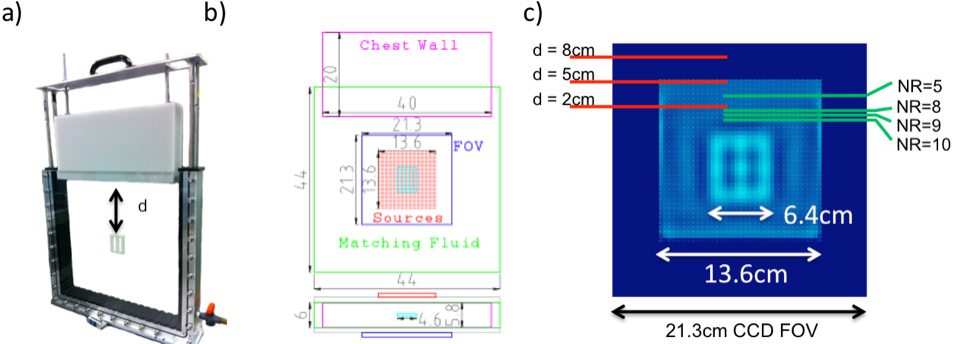
\includegraphics[width=\textwidth]{./figures/chestwall_3.pdf}
\caption{\label{fig:data}
  Models for data restriction. (a) Photograph of the drained imaging
  tank illustrating the position the target with respect to the chest
  wall phantom. (b) Schematic of the imaging tank. (c) Illustration of
  the various data sets used in the reconstructions. The dark blue
  square is the CCD FOV while the inner light blue square indicates
  the reconstruction region. The bright dots indicate the source
  positions. A sample reconstruction is superimposed with the drawing
  to illustrate the target shape and position. The red lines indicate
  the three lowest position of the chest wall phantom (other positions
  are outside of the CCD FOV) while the green lines illustrate the
  restricted data sets where all the sources and detectors situated
  above a given green line have been discarded.}
\end{figure}

\begin{table}[t]
\centering\caption{Data Restriction Sizes.}
\begin{tabular}{c|c|c}
\hline 
Numerical data Restriction ($NR$) & Number of sources & 
Number of distinct \\
&& source-detector pairs \\ \hline
No restriction & $35\times35=1225$ & $20591492$ \\
           $5$ & $35\times31=1085$ & $16479152$ \\
           $8$ & $35\times28=980$  & $14661145$ \\
           $9$ & $35\times27=945$  & $14074728$ \\
          $10$ & $35\times26=910$  & $13457507$ \\ \hline
\end{tabular}
\end{table}

\section{Results}
\label{sec:res}

The quantity plotted in all figures of this section is $x({\bf r}) + 1 = \alpha({\bf r}) / \alpha_0$. From physical considerations, this function is nonnegative, since the medium is not amplifying.  However, the image reconstruction reported here utilizes various approximations. This can result in reconstructing unphysical negative values of absorption, which are shown in the figures by the color black (the same color scale is used throughout). We note that the
occurrence of negative absorption can be avoided by making use of a positivity constraint in the algebraic reconstruction method. The positivity constraint can be incorporated in the conjugate-gradient descent algorithm, which was used by us to invert the matrix $A^*A$. However, we have found that the areas of negative absorption appear mostly in the case of the analytic (fast) image reconstruction method, which cannot incorporate the positivity constraint. On the other hand, the algebraic reconstructions have produced either no areas of negative absorption, or artifacts so severe (e.g., when $d=2\,{\rm
  cm}$ and no numerical data restriction) that the use of the positivity constraint was not useful. In other words, we did not encounter a situation in which the positivity constraint was simultaneously numerically feasible and useful; therefore, it has not been used for producing the images shown in this section.

Reconstructions of the central slice of the medium ($3\,{\rm cm}$ from either of the slab surfaces) obtained with varying values of $d$ and various numerical data restriction ($NR$) are shown in Fig.~\ref{fig:central}. It can be seen in Fig.~\ref{fig:central}(a) that the analytical inversion with no data restriction (the topmost row of images) produces severe image artifacts when chest wall is $d=2\,{\rm cm}$ and $d=5\,{\rm cm}$ away from the target. Data restriction with $NR=5$ results in a reasonable, yet suboptimal, image quality when $d=5\,{\rm cm}$, but not when $d=2\,{\rm cm}$. To remove
the artifacts associated with the chest wall completely, $NR=10$ is required.

However, $NR = 8,9,10$ used in conjunction with the analytical reconstruction yields an additional image artifact, which is unrelated to the chest wall phantom. To see that this is true, consider the images for $d=17\,{\rm cm}$, which are not affected at all by the chest wall phantom, yet exhibit the additional artifact just mentioned. This artifact is shown as a black area where the reconstructed absorption coefficient is negative and, therefore, outside of the physically-allowable range. We thus conclude that reconstructing the target by the analytical reconstruction method is feasible with the use of the appropriate data restriction, yet it results in an additional image artifact where the absorption in underestimated. 

The appearance of this artifact can be understood. As mentioned above, the data restriction used with the analytical reconstruction amounts to assuming that the truncated data points are zero. In other words, we assume that, in the presence of the target, the truncated source-detector pairs would have measured the same intensity as in the homogeneous slab, so that $I({\bf r}_d,{\bf r}_s) = I_0({\bf r}_d,{\bf r}_s)$ for the truncated source-detector pairs
(see Eq.~(\ref{eq4})). The reconstruction algorithm seeks a contrast function $\delta\alpha({\bf r})$, which is compatible with this assumption.  For a purely absorbing target, however, the actual intensity $I({\bf r}_d,{\bf r}_s)$ is smaller than $I_0({\bf r}_d,{\bf r}_s)$ when at least one of the points ${\bf r}_d,{\bf r}_s$ is located not too far from the target (in the lateral direction) due to increased optical absorption. Whenever such data points are discarded,
an artifact with negative $\delta\alpha$ is produced by the reconstruction algorithm to compensate for the absorption in the target. It can be seen that this artifact is located between the target and the region of source-detector pairs, which have been discarded. Of course, this analysis applies to the case when the position and optical contrast of the target is known.  In general, it may be difficult to predict the position of this artifact or to distinguish it from a true occurrence of negative $\delta\alpha$. There may also be a spatial overlap of the artifact and a true inhomogeneity.

We now turn to the algebraic reconstructions [Fig.~\ref{fig:central}(b)]. For the unrestricted data set, the image quality is still poor. However, when the data restriction is gradually introduced, the artifacts disappear.  Thus, in the case $NR=10$ and $d=2\,{\rm cm}$ (the image in the bottom right corner), the target is clearly visible, and the image quality is about the same as with the use of the unrestricted data set and $d=17\,{\rm cm}$. Thus, introduction of the data restriction does not result in additional image artifacts or quality degradation when the algebraic method is used.

In Figs.~\ref{fig:slices_analytical} and \ref{fig:slices_numerical}, we show slices drawn through the medium at different depths. Fig.~\ref{fig:slices_analytical} displays the results of the analytical image reconstruction for $d=5\,{\rm cm}$ and $d=2\,{\rm cm}$ and Fig.~\ref{fig:slices_numerical} displays analogous data obtained by the algebraic reconstruction. In addition, we show in the right-most column of images the reconstruction averaged over the depth of the sample (that is, over different slices). Note that all reconstructed slices were used for the purpose of averaging, not only those shown in the figures. Note that, in all cases, we have reconstructed $13$ slices separated by the distance of $8h\approx 3.328{\rm mm}$, with the central slice located exactly in  the mid-plane of the slab. The ``average'' reconstruction was  obtained by computing the arithmetic average of the reconstructions in all $13$ slices. These averaged (``projection'') images correspond to the usual radiological projections obtained with a parallel beam of X-rays. The qualitative conclusions that can be drawn from Figs.~\ref{fig:slices_analytical} and \ref{fig:slices_numerical} are the same as above. The analytical reconstruction produces reasonable image quality for the smallest chest wall-target separation $d=2\,{\rm
  cm}$ and $NR=10$ but at the cost of an additional image artifact.The algebraic reconstruction is free from this artifact, but underestimates the image contrast relative to the analytic method (see below). The depth resolution is slightly better in algebraic reconstructions but, overall, much worse than the lateral resolution. This is typical for DOT images.

One interesting feature observed in both types of image reconstruction is the following. The projection images discussed above are, generally, more stable and exhibit reasonable quality even when the individual slices contain severe artifacts. For example, consider the $d=2\,{\rm cm}$ algebraic reconstructions without data restriction (Fig.~\ref{fig:slices_numerical}). Even though all slices drawn through the medium are badly corrupted by the artifacts associated
with proximity of the chest wall phantom, the projection image shows the target clearly. Moreover, the edge of the chest wall phantom is also clearly visible at the correct location. This result is somewhat unexpected and can be useful in the situations when the depth resolution is not of essence. We emphasize that obtaining the projections still requires knowledge of the three-dimensional distribution of the absorption coefficient; the projections cannot be computed or measured directly without such knowledge.

We note that, in both types of image reconstructions, we see an underestimation of the contrast for the target phantom compared to the expected value. This underestimation can be attributed to the poor  transverse (depth) resolution of the three-dimensional reconstruction which results in the ``spreading'' of the contrast in that direction. Indeed, consider the depth-integrated contrast, $H(x,y) = \int \left[  \alpha(x,y,z) / \alpha_0 - 1 \right] {\rm d}z$, where $x$, $y$ are the coordinates in the plane of the slab and $z$ is the transverse (depth) coordinate. Inside the target, we have $\alpha(x,y,z) / \alpha_0 \simeq 4$ and the target thickness in the transverse direction is $\Delta z=0.6\,\ {\rm cm}$. Therefore, the actual value of $H$ for a line passing through the target and perpendicularly to the slab surface is $H\simeq 1.8\,{\rm cm}$. In the reconstructed images, the transverse thickness of the target is overestimated and is equal, approximately, to $2\,{\rm cm}$ while the quantity $\alpha(x,y,z)/\alpha_0$ is underestimated and is equal, approximately, to 2. By using the reconstructed values to estimate the integrated contrast, we obtain $H\simeq 2\,{\rm cm}$, which is reasonably close to the actual value.

\begin{figure}[htbp]
\begin{center}
\begin{minipage}[h]{1\textwidth}
\begin{center}
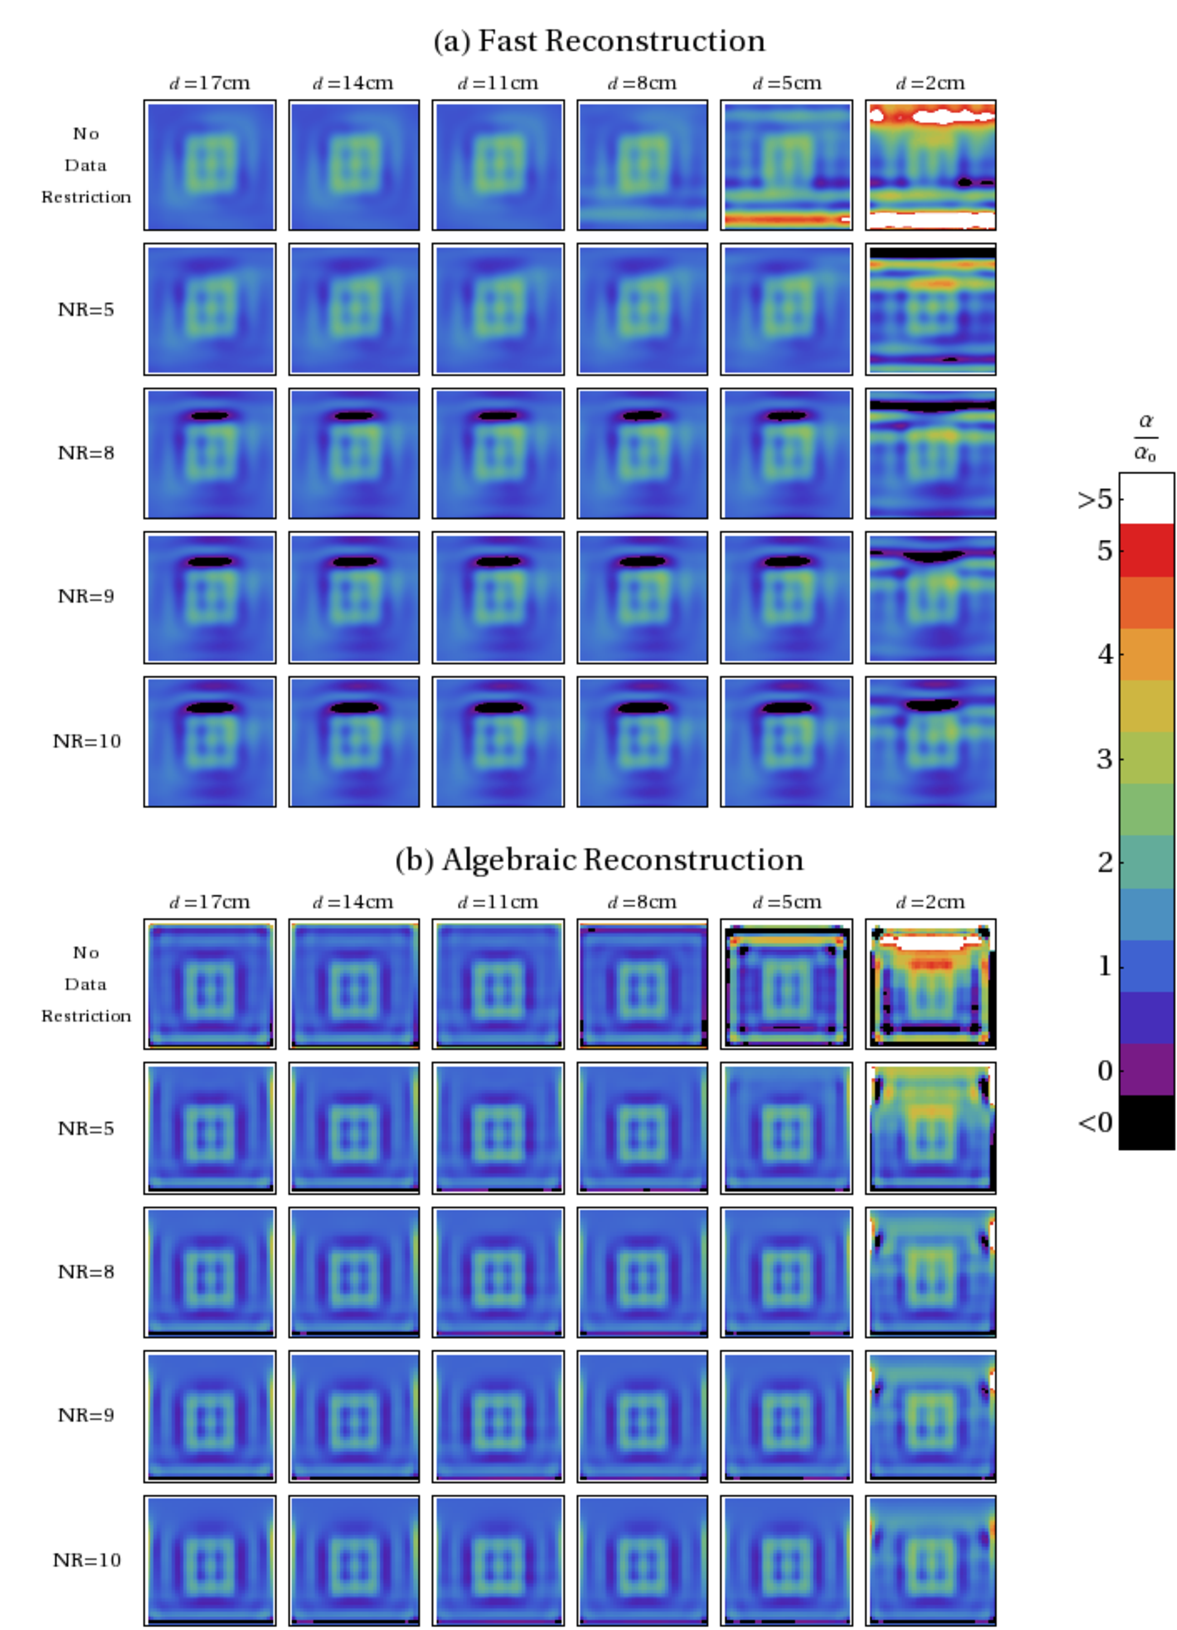
\includegraphics[width=0.85\textwidth]{./figures/chestwall_4.pdf}
\end{center}
\end{minipage}
\end{center}
\caption{\label{fig:central}
  Images of the central slice obtained by analytical (a) and algebraic
  (b) reconstruction methods. Different columns show data obtained
  with the chest wall phantoms at different distances $d$ from the bar
  target.  Different rows of images correspond to different data
  restrictions $NR$, as indicated.  The color bar applies to all other
  images shown below.}
\end{figure}

\begin{figure}[htbp]
\begin{center}
\begin{minipage}[h]{1\textwidth}
\begin{center}
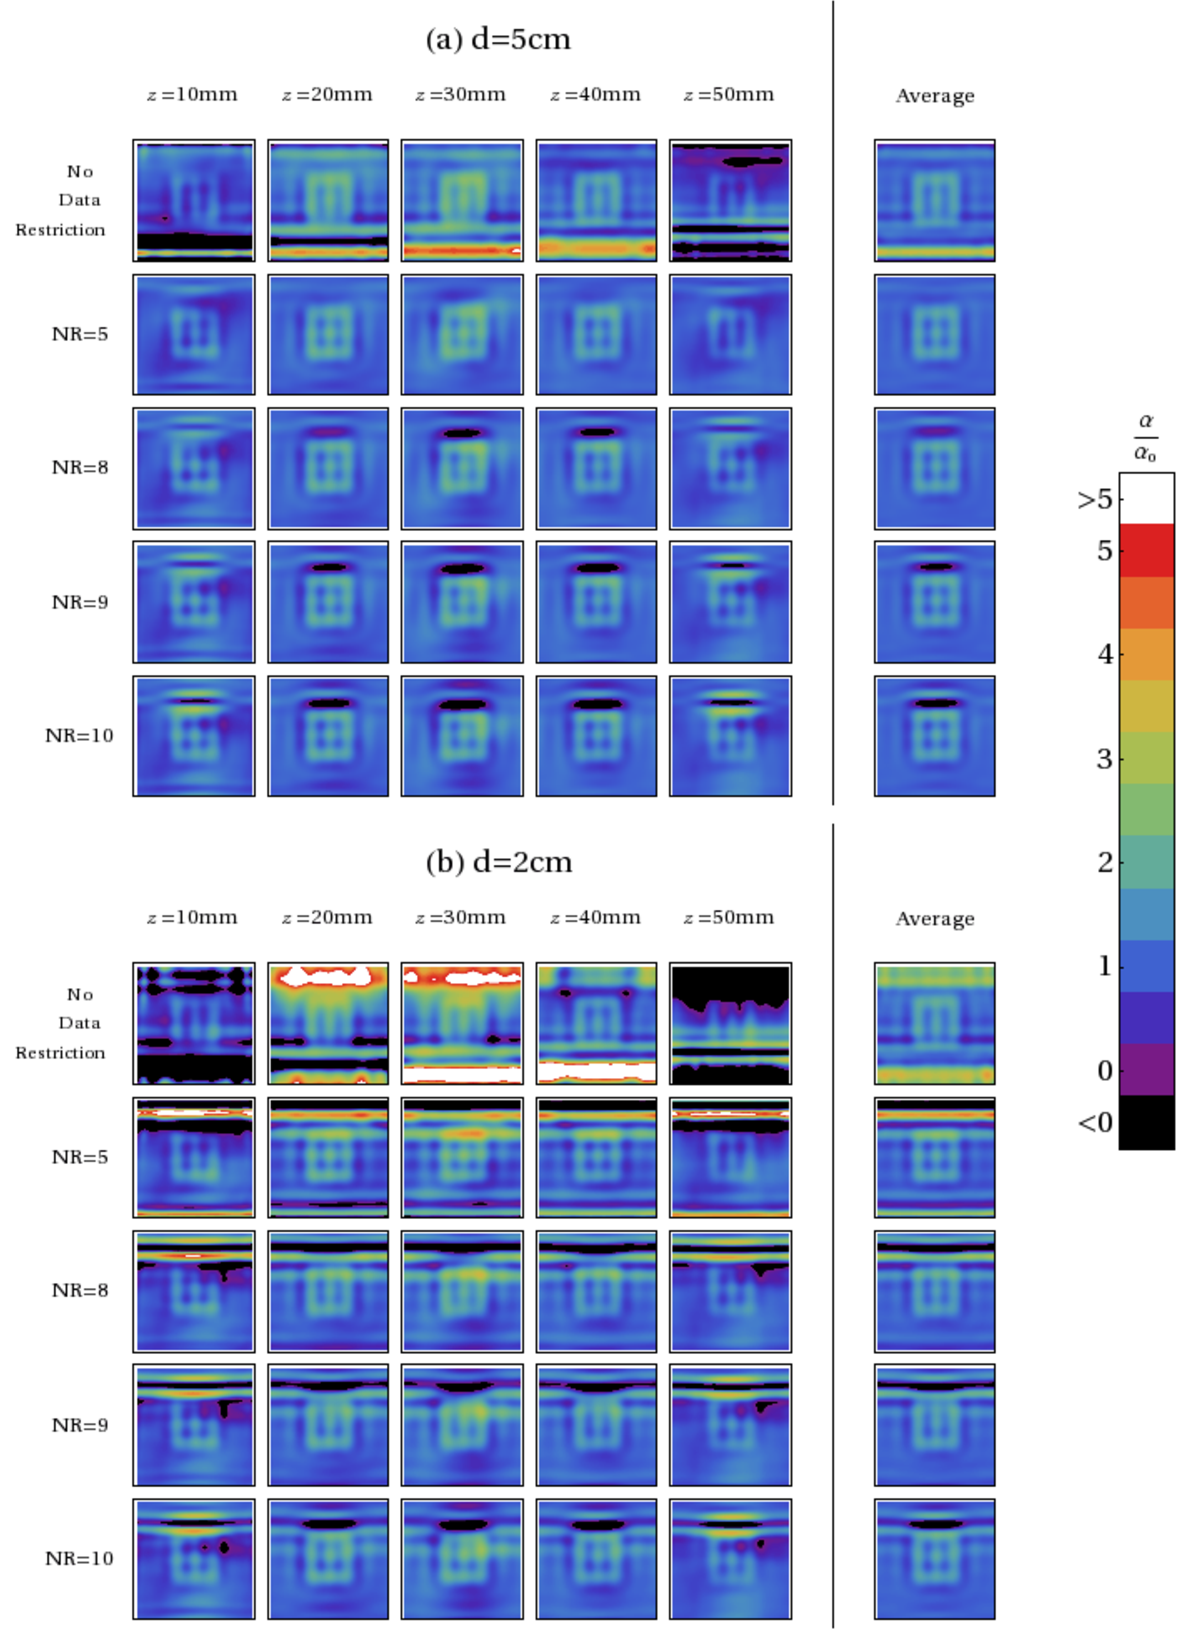
\includegraphics[width=0.9\textwidth]{./figures/chestwall_5.pdf}
\end{center}
\end{minipage}
\end{center}
\caption{\label{fig:slices_analytical}
  Slices through the medium drawn at different depths (from the plane
  of sources) as indicated. Analytical image reconstruction method
  with $d=5\,{\rm cm}$ and $d=2\,{\rm cm}$.}
\end{figure}

\begin{figure}[htbp]
\begin{center}
\begin{minipage}[h]{1\textwidth}
\begin{center}
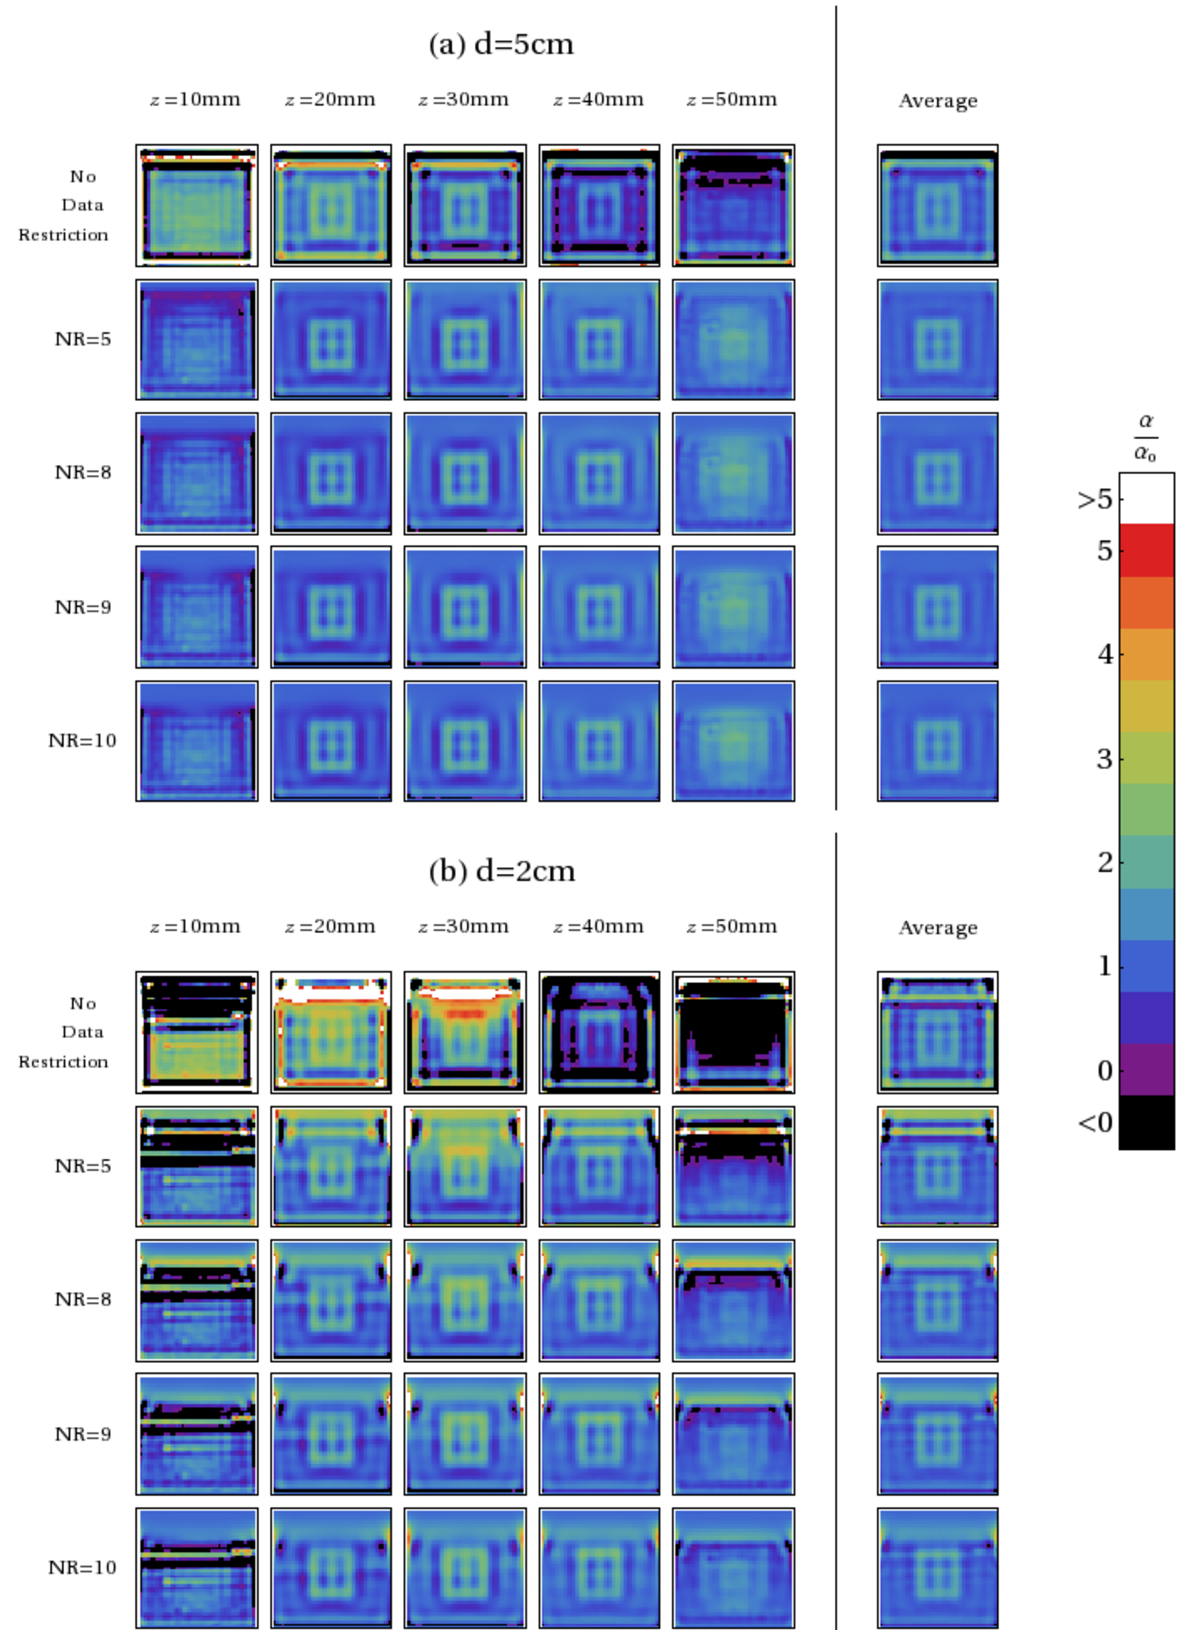
\includegraphics[width=0.9\textwidth]{./figures/chestwall_6.pdf}
\end{center}
\end{minipage}
\end{center}
\caption{\label{fig:slices_numerical}
  Same as in Fig.~\ref{fig:slices_analytical} but obtained by
  algebraic reconstruction. }
\end{figure}

\section{Summary and discussion}
\label{sec:sum}

We have used phantom experiments to investigate systematically the effects of the chest wall on diffusion optical tomography (DOT) of the breast.  The results lead us to several promising conclusions. 

First, we have found that, when absorption contrast is of interest, simple continuous-wave instrumentation with linearized inversion can suffice. This finding was obtained in spite of the presence of the chest wall phantom in close proximity to the target, which (i) renders the inverse problem nonlinear and (ii) differs from the background Intralipid and the target not only in absorption but also in scattering properties.  Generally, under the conditions stated above,
time- or frequency-resolved measurements and nonlinear image-reconstruction methods are required. We, however, have been able to bypass these complications by appropriately restricting the data points used in the reconstruction. We note that in clinical applications of DOT, the location of the chest wall relative to the sources and detectors is usually known;  therefore, the approach of this paper to data restriction can be applied {\em in vivo}. Work remains,however, to optimize these approaches. Devising the latter, for example, may require more sophisticated and/or data-driven algorithms for data rejection, as well as  experimentation {\em in vivo}. In this paper, we have demonstrated that the rather severe effects of the chest wall can, in principle, be rectified by appropriate data restriction in conjunction with a linear image reconstruction. The paper shows that, by means of properly restricting the data points used in image reconstruction, it is possible to resolve a small absorptive target in the vicinity of a spatially and optically large inhomogeneity
and that the quality of the reconstruction is almost unaffected by the chest wall.

Interestingly, we have also found (see Figs.~5 and 6) that the image contrast, when averaged over the depth of a plane-parallel sample (we refer to
this quantity as the projection), is not as sensitive to systematic errors encountered in image reconstruction as the individual slices drawn through the medium. Thus, under certain conditions, the nonlinearity of the inverse problem and the presence of a scattering contrast render our image reconstruction methods inadequate. Reconstructed slices show severe image artifacts in this case. The projection, however, is free from these artifacts and displays the target clearly. This finding may be significant since a projection of the type just discussed is similar to the usual radiographic projection, yet it displays the contrast specific to the near-infrared spectral range.

Finally, we have developed and verified with experimental data an algebraic image reconstruction method, which is well suited for the use with the data 
sets restricted by the presence of the chest wall and capable of handling data sets as large as $2\times 10^7$ independent measurements.